\pdfoutput=1
\documentclass[12pt]{article}
%%%% LOAD PACKAGES
% Remove the indentation when starting new paragraphs, but still add a blank line.
\usepackage[parfill]{parskip}
\setlength{\parindent}{0pt}
\setlength{\parskip}{\baselineskip}
% Package for dealing with graphics - for figures.
\usepackage{graphicx}
% use the , as a thousand unit separator
\usepackage{numprint}
\npthousandsep{,}
%to multiplication and division
%\usepackage{calc}
\usepackage[nomessages]{fp}
%Font of mathematical symbols 
\usepackage{MnSymbol}
%is a modified tabular* allowing width of columns set for equal heights
\usepackage{tabulary}
%provides the command needed for spanning rows:
\usepackage{multirow}
%to insert url without using the package hyperref
\usepackage{url}
\urlstyle{same}
% Switch from the default font to Times as default is very thin
\usepackage{times}
% Allows a space to be included after inserting formatted text.
\usepackage{xspace}
% Allow single pages to be changed to landscape, including in PDF preview.
\usepackage{lscape}
% More formatting options for lists
\usepackage{enumitem}
% Set the margin width - this will need changing to account for having uneven borders for binding.
\usepackage[top=2.45cm,bottom=2.45cm,left=3.17cm,right=3.17cm,twoside]{geometry}
% Allow figures and tables to be named in different ways.
\usepackage{chngcntr}
% Allow Harvard formatting for references - reference with \citepp{key,key2,etc.}.
% Remember that you have to run Macros -> Applescript -> Bibliography (?r) to make references appear
% The style file for this is referred to in the section at the bottom.
\usepackage{natbib}
\setlength{\bibsep}{0.0pt}
\bibpunct{(}{)}{;}{a}{,}{,}
% First line adds the reference section to the Contents page, second line renames it from 'Bibliography' to '4References'
%\usepackage[nottoc,numbib]{tocbibind}
\usepackage[nottoc]{tocbibind}
\settocbibname{References}
%use this package to reference the figures and tables in the supplemental file 
%use this package to highlight certain cells in a table
\usepackage[table]{xcolor}
\usepackage[nodayofweek]{datetime}
\usepackage{setspace}
\usepackage{authblk}
\usepackage{lineno}
\usepackage[group-separator={,}]{siunitx}
\usepackage{hyphenat}
\usepackage{tikz}
\usepackage{fmtcount}
\DeclareSIUnit{\molar}{M}
\usepackage{subfig}
\usepackage{hyphenat}
\usepackage{seqsplit}
\usepackage[font={footnotesize }]{caption}
\usepackage{xr}

% Douda's additions
\usepackage{supertabular,multirow}
\usepackage[flushleft]{threeparttable}

\externaldocument{robinson_etal_distr}


\renewcommand{\seqinsert}{\ifmmode\allowbreak\else\-\fi}
  
%%%% DOCUMENT FORMATTING %%%%
% Format the document with 1.5 line spacing.
\onehalfspacing

%%%% DOCUMENT VARIABLES %%%%
\input{results_latexDB.txt}

\begin{document}


%%%% SUPPLEMENTAL RESULTS %%%%
\section*{Supplemental Results}
\label{sec:Supplemental Results}

\subsection*{Identification of \textit{Candida albicans} from oak trees in the New Forest, UK}
\doublespacing

The human commensal and pathogenic yeast species \textit{Candida albicans} has only rarely been isolated from natural environments that are not associated with mammals \citep{tanghe_aquaporin_2005,lachance_chapter_2011-5,maganti_ecological_2011}. Here we isolated three yeast strains from northern European oak trees with rDNA sequences, identical to several different isolates of \textit{C. albicans} (site 6 in Figure 1 and Table 2) that were isolated from humans around the world (Supplemental File 2). All three rDNA sequences from these strains differed (by at least 15 nucleotides) from the type strain of the most closely related species \textit{C. dubliniensis} \citep{lachance_chapter_2011-5} suggesting that these are indeed \textit{C. albicans}, and that it occurs in this natural habitat. We note that \textit{C. albicans} was isolated from three of the oldest oak trees sampled in this study (trunk girth, 2.8-4.1m). 

A few lines of evidence suggest that these strains do not represent human commensal contaminants introduced  during sample processing. To avoid sample contamination (and exposure of workers to unidentified microbes), all samples were processed in a class II cabinet. Additionally, negative controls generated in the field generated no colonies after enrichment culturing. Similarly, all negative controls associated with DNA extraction and PCR amplification of these samples were also blank, and identical rDNA sequences were generated by two different lab members. Two of the rDNA sequences associated with the three different \textit{C. albicans} differ by an unambiguous single nucleotide insertion or deletion, therefore at least 2 distinct contaminants would be needed to explain this diversity.

If ancient oaks do indeed represent a natural habitat of \textit{C. albicans} however, it must be rare in this environment because we isolated it from only one site out of 13. Furthermore, others have isolated other \textit{Candida} species from trees but not \textit{C. albicans}, suggesting that they could have recovered \textit{C. albicans} if it was present at appreciable frequencies \citep{maganti_ecological_2011,charron_exploring_2014,sylvester_temperature_2015}

\subsection*{The ecological niche of \textit{S. cerevisiae}}

In order to test whether \textit{S. cerevisiae} is more abundant on fruits than on other substrates, we compared \textit{S. cerevisiae} isolation rates between fermenting grape must ($n=\must$), grapes ($n=\vineyardgrape$), grape vine bark ($n=\grapebark$) and oak bark ($n=\vineyardoakbark$) samples in two UK vineyards after the grape harvest. As expected, \textit{S. cerevisiae} is isolated more readily from fermenting grape must samples (\scmustpcent\%) than it is from grape samples (\scgrapepcent\%; Fisher's exact test, $P=\fishergrapemust$), but \textit{S. cerevisiae} isolation rates from grapes are very similar to those for grapevine bark (\scvinebarkpcent\%; Fisher's exact test, $P=\fishergrapebark$) and oak bark (\scvineyardoakbarkpcent\%; Fisher's exact test, $P=1$). 

Likewise, fig trees in Southern Europe showed similar \textit{S. cerevisiae} isolation rates from fig tree bark (\scfigbark\ out of \figbark, \scfigbarkpcent\%) and figs (\scfigfig\ out of \figfig, \scfigfigpcent\%; Fisher's exact test, $P=\fisherfigbark$). Although it was difficult to quantify, we noticed that unripe figs may have lower rates of yeast isolation, and our sampling of unripe fruit could contribute to the low overall \textit{S. cerevisiae} rate from figs. Fig tree bark may therefore provide a more stable substrate for yeast isolation, especially where trees are old.


\subsection*{Differences among trees in the prevalence of \textit{Saccharomyces paradoxus}}

This study generated data for \oakbarknotten\ bark samples from \treecount\ different oak trees that were tested for the presence or absence of \textit{S. paradoxus} by enrichment culture at 25 or 30\si{\degreeCelsius}. In most cases (\treessampledfourtimes\ trees), 4 pieces of bark were sampled from the same tree, and \repeatedtrees\ trees were revisited in different months (June-September, and November) and years (2006-2011). 

To test whether the probability of isolating \textit{S. paradoxus} differs among trees, and for possible effects of sample weight or time of collection, we used logistic regression (GLM with binomial errors) to model the presence or absence of \textit{S. paradoxus} in each bark sample (a binary response variable). The initial model included a factor to describe the effect of each oak tree (\treecount\ levels), a second factor for collection month (5 levels: June-September, November), weight (in grams) as a continuous variable, and the two-way interaction between weight and collection month. This full initial model was simplified by subtracting terms in a stepwise manner starting from the two-way interaction and testing whether each subtraction resulted in a worse model using $\chi^2$ tests as recommended in \citet{crawley_statistics:_2005}.

In this analysis, bark weight was not a good predictor of the presence or absence of \textit{S. paradoxus} (GLM, -\weightpcentdev\% deviance, $d.f.=\weightdf, P=\weightp$). There was also no obvious difference in isolation rates in different months (GLM, -\monthpcentdev\% deviance, $d.f.=\monthdf, P=\monthp$). This can be explained by the fact that most samples (75\%) were collected between 25th August and 7th September. There were, however, clear differences among trees in the likelihood of \textit{S. paradoxus} isolation from their bark, which explain \treepcentdev\% of the variation among samples (GLM, $\chi^2=, d.f.=\treedf, P=\treep$). 

Because weight and collection month do not have a significant effect on \textit{S. paradoxus} isolation frequency, we were able to pool data for multiple bark samples from each oak tree in the main analysis, and therefore to use the proportion of bark samples from each tree that resulted in \textit{S. paradoxus} isolates as a response variable (see Methods). This was preferable to using a binary response variable with several different explanatory variables, which would result in fitted probabilities of zero or one in the final model, and these lead to known problems with binomial GLMs \citep{venables_modern_2002}. 

\subsection*{Choice of laboratory study to estimate the difference between \textit{S. paradoxus} and \textit{S. cerevisiae} in optimal growth temperature}

We rely on an accurate estimate in the difference between optimal growth, but studies that compare \textit{S. paradoxus} and \textit{S. cerevisiae} measure the difference approximately \citep{liti_population_2009,leducq_local_2014} or disagree in the extent of the difference (2\si{\degreeCelsius}, \citealp{salvado_temperature_2011}; 7\si{\degreeCelsius}, \citealp{sweeney_sympatric_2004}). We chose to use the study by \citet{sweeney_sympatric_2004} because (i) they screen many strains from both \textit{S. paradoxus} and \textit{S. cerevisiae} that were isolated from oak trees and oak trees are also the focus of this study; (ii) their growth profiles are typical for each species \citep{liti_population_2009}; and (iii) their estimate is closer to the observation by \citet{leducq_local_2014} that type strains for \textit{S. cerevisiae} and \textit{S. paradoxus} differ by approximately 10\si{\degreeCelsius}. In addition, the \textit{S. paradoxus} strains used by \citet{sweeney_sympatric_2004} have a North American genotype (\textit{SpB}; \citealp{kuehne_allopatric_2007}) that suggests they may grow better at high temperatures than \textit{S. paradoxus} strains with a European genotype \citep{leducq_local_2014,leducq_speciation_2015}. It is therefore possible that \citet{sweeney_sympatric_2004} underestimate the difference between \textit{S. cerevisiae} and \textit{S. paradoxus} in optimum growth temperature.

How would our results differ if we had chosen to use a different estimate \citep{salvado_temperature_2011} from fewer strains of \textit{S. paradoxus} and \textit{S. cerevisiae} mostly isolated from fruit? \citet{salvado_temperature_2011} report a \textit{S. cerevisiae} optimum 2\si{\degreeCelsius} higher than \textit{S. paradoxus} and a maximum temperature for growth that is 4\si{\degreeCelsius} higher. If we assume a 4\si{\degreeCelsius} difference, then this correctly predicts the presence of \textit{S. cerevisiae} isolates with wild genotypes, but does not explain why only human-associated strains or those approximately mapping to mountains are isolated between 22\si{\degreeCelsius} and 25\si{\degreeCelsius} (Figure 5, Supplemental Figure \ref{fig:china}) or why no \textit{S. cerevisiae} were isolated in the southern UK (23\si{\degreeCelsius}, \citealp{johnson_population_2004}) or Canada (T$_{max}$ 25\si{\degreeCelsius}, \citealp{charron_exploring_2014}).

%\subsection*{Geographic distance and prediction of \textit{S. paradoxus} isolation frequency}

%The field sites in this study lie in a north-south gradient within Europe. This raises the possibility that summer temperatures (T$_{max}$) could correlate with geographic distance and therefore many other factors that might better explain differences among trees in \textit{S. paradoxus} isolation frequency. We estimated the geographic distance of each tree from the northernmost tree by applying the simple distance formula: $d=\sqrt{(x_{n}-x_{i})^2+(y_{n}-y_{i})^2}$, where $x_{i}$ and $y_{i}$ are the longitude and latitude coordinates for each tree, and $x_{n}$ and $y_{n}$ are the coordinates of the northernmost tree. To test the possibility that geographic distance explains differences among trees in \textit{S. paradoxus} isolation frequency, we used our measure of geographic distance to predict the proportion of bark samples with \textit{S. paradoxus} for each tree in a GLM (with binomial errors) together with oak trunk girth, north-south, and T$_{max}$. Distance did not explain the differences in \textit{S. paradoxus} isolation frequency as well as the other explanatory variables and was dropped from the model after standard model simplification \citep{crawley_statistics:_2005}. In addition, replacing either the north-south explanatory variable or T$_{max}$ with distance resulted in worse models (AIC=\textcolor{red}{173} and AIC=\textcolor{red}{193}; compared to the final model AIC=\textcolor{red}{155}).

\clearpage

%%%% SUPPLEMENTAL TABLES AND FIGURES %%%%
\section*{Supplemental Tables and Figures}
\label{sec:Supplemental Tables and Figures}

\setcounter{table}{0}
% change the name of the tables to supplemental tables 
\renewcommand{\tablename}{Supplemental Table}

% Supplemental Table 1
\begingroup
\renewcommand*{\thefootnote}{\alph{footnote}}
\begin{table}[h!] \centering 
 \begin{threeparttable}
\caption{{\bf Primers used to identify yeast species by PCR and DNA sequencing }} 
      \label{tab:scsp_table}
\begin{tabular}{llp{1cm}p{1.3cm}l} \hline
Species & Locus & PCR name & Primer name & Primer sequence \\ \hline
Saccharomycetales & rDNA\footnote\ & ITS & ITSf1 & AAAGTCGTAACAAGGTTTCCGTAG \\
  &  &  & ITSr & TCCGCTTATTGATATGCTTAAGTTC \\
 &  & ITS2 & ITSf2 & GAAsTAAAAGTCGTAACAAGGTTTCC \\
 &  &  & ITSr & TCCGCTTATTGATATGCTTAAGTTC \\
 &  & S1L & S1Lf & ATTTGAGGTCAAACTTTAAGAACATTG \\
 &  &  & S1Lr & AGAGGAACTAAAAGTCGTAACAAGG \\
\textit{Saccharomyces} & CEN6 & cepC6\footnote\ & cepC6f & GAACCTGTCGAAGTTGTTAATGC \\
  &  &  & cepC6r & TrGAAGGTTTCTTTGGwGCCAT \\
  &  & parC6\footnote\ & parC6f & CGAAGTTGTTAATGCGAAATATTCTA \\
  &  &  & parC6r & ACCTCTCTTCTCAAAGTTTGCCT \\
 \textit{S. paradoxus} & CEN9 & parC9 & parC9f & ATATTCTAGCCGATCTGGAACTTG \\
  &  &  & parC9r & CAGATAACGTTAAAAGTTCTGTCCAA \\
  & CEN15 & parC15 & parC15f & TCATATTTATAACAAGCGATCAAAGC \\
  &  &  & parC15r & GAAGTACATCCTGATTTTTAGAAGCC \\
\hline
\end{tabular}

    \begin{tablenotes}
      \small
      \item See \citet{bensasson_evidence_2011} for details of the three primer pairs (cerC6, cerC9 and cerC15) used for \textit{S. cerevisiae}-specific amplification of centromere loci. 
      \item [a] Primers anneal to 18SrRNA and 25SrRNA, and amplify all of ITS1-5.8SrRNA-ITS2 (see Methods). 
      \item [b] Amplifies \textit{S. cerevisiae}, \textit{S. paradoxus}, and \textit{S. kudriavzevii} DNA, but with a product of a different size for \textit{S. kudriavzevii}. 
      \item [c] Amplifies \textit{S. paradoxus} and \textit{S. kudriavzevii} DNA, but with a product of a different size for \textit{S. kudriavzevii}.      
     \end{tablenotes}
 \end{threeparttable}
\end{table}
\clearpage

\setcounter{figure}{0}
% change the name of the figures to supplemental figure 
\renewcommand{\figurename}{Supplemental Figure}

% Supplemental Figure 1
\begin{figure}[h!] \centering
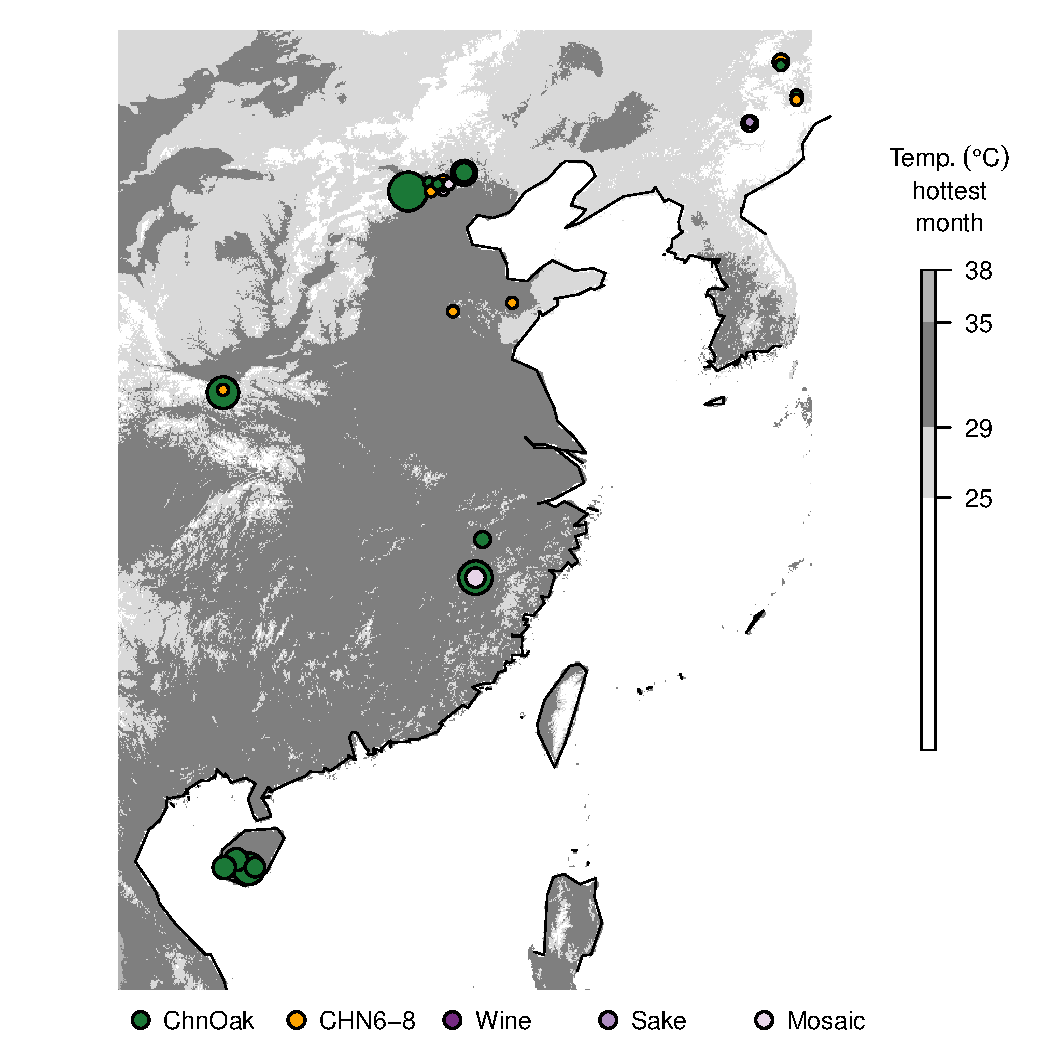
\includegraphics[width=1\textwidth]{../figs_tables/FigureS1China.pdf}
\caption{{\bf Approximate geographic positions of \suppfigstrains\ \textit{S. cerevisiae} strains from China are close to locations with expected summer temperatures.} Regions shaded in grey show summer temperatures that we predict are optimal for \textit{S. cerevisiae}. Approximate collection sites described in \citet{wang_surprisingly_2012} are shown with points scaled by the square root of sample size. Strains with genotypes that are associated with humans are shown in purple, and mosaic strains show recent admixture between multiple populations. Strains with genotypes that are so far only associated with woodlands are shown in green (CHNI, CHNII, CHNIII, CHNIV, CHNV), strains with genotypes that are more similar to those seen in other parts of the world are shown in orange (CHNVI, CHNVII, CHNVIII) and all of the approximate isolation sites for these are close to locations with the optimum summer temperature (T$_{max}$) for \textit{S. cerevisiae}. }
\label{fig:china} 
\end{figure}
\clearpage

%%%% REFERENCES %%%%
\bibliographystyle{final}
{\footnotesize \linespread{1}
\bibliography{../../../labbibtex/bensassonlab.bib}}
\clearpage


\end{document}